\ifdefined\included
\else
\setcounter{chapter}{7} %% Numéro du chapitre précédent ;)
\dominitoc
\faketableofcontents
\fi

\chapter{Moving forward binary relations in the REG}
\minitoc

The contribution presented in this chapter is a preliminary work aiming to consider the limitations encountered by the contribution of the previous chapter. The presented method has been implemented but not tested with an integration of other components. This section deviates a little from the field of HRI to be more anchored in artificial intelligence. However, the ability to generate entity referencing in a more generic way is paramount for a robot to interact with humans. 

\section{Introduction}

Representing the whole complexity of the knowledge composing our world into a machine-readable language is a central issue in artificial intelligence. Coming from the Semantic Web, we saw that the use of an ontology through RDF-based languages succeeded in establishing itself in the field of artificial intelligence and therefore robotics. Although, what is often viewed as a limitation of ontology is its capability to only represent unary and binary relations. Binary relations such as \textit{"Sean Connery has the British nationality"} are described through the form of triples \textit{(sean\_connery, hasNationality, british)}. Unary relation such as \textit{"Sean Connery is an actor"} can them be transformed into binary relation through the addition of dedicated predicates \textit{(sean\_connery, isA, Actor)}. However, the description of more complex relations involving more than two entities is must more challenging using such representation.

Taking the example of Sean Connery\footnote{In the case you do not know who is Sean Connery feel free to take another actor that you like but you will have to adapt the entire example. Good luck.}, f we want to refer to him\footnote{Obviously we want to refer to him without his name since we consider a person having recognized himself in the previous note.}, we could state that he is the actor playing the role of James Bond. However, other actor played this role. We could also say that he is the actor playing in the film Gold finger but once again others do. We could finally explain that he is the actor playing the role of James Bond and playing in the film Gold Finger. However, limiting us to the use of binary relations modify the exact information. A more accurate description would be that he is the actor playing the role of James Bond in the film Gold Finger. Here we see the necessity of relations involving more than two entities. In our example, we need to link the three entities that are the actor "Sean Connery", the role "James Bond", and the film "Gold Finger". Together, they describe a performance. Without being explicitly linked all three theses information would not represent the performance. Moreover, without these links, we could give an explanation such as the actor playing the role of James Bond and playing in the film Rising Sun. Both information is true but does not make sense together.

To refer to an entity, being an object or an agent, such complex relations could be useful but have to be managed carefully to keep the link between each binary relation composing it. In the light of this consideration, we can observe that the description of past agent tasks used in the previous chapter is based on the same principle. Where we refer to Sean Connery through his role and the film he plays in, we have described the knife through the vegetable it has been to cut and the agent having used it. However, depending on the context of the conversation, is it not always necessary to use all the binary relations of such a complex one. We may need only one. Trying to list the actors having the honorific title of "Sir", the referring expression \textit{"The man having played James Bond"} could be sufficient. In the same way, to designate the knife, the sentence \textit{"The knife you cut with"} could also be sufficient in some context.

In this chapter, we will try to generalise the REG algorithm to deal with non-binary relations and pass over the limitations of the previous chapter. The algorithm has to be more generic should no more have any apriori of concepts and properties of the used ontology.
First, we review the literature concerning the representation of non-binary relation in the ontology. Then, we define what we will call a Compound Relation and how we can represent it. The modified algorithm is then detailed before ending with an efficiency comparison regarding the original version and the extended one.

\section[Related work]{Related work: A richer knowledge representation with n-ary relations}

A fundamental feature of relations is their \textbf{arity}. It is the number of individuals they involved~\cite{giunti_2019_representing}. In this sense, unary relations involved only one entity while binary relation involves two entities\footnote{The entities involved in a relation do not have to be distinct. If the same entity is used twice in the same relation the relation is still a binary relation}. What interest us here is n-ary relations with arity $n > 2$.

Well before being treated for ontology used that it is in RDF or OWL, several approaches have been proposed in the field of Artificial Intelligence through the use of semantic network\footnote{Here we close the loop with the hypothesis by Collins and Quillian of the structure of the semantic memory to be like a semantic network.}~\cite{brachman_1979_epistemological, sowa_2014_principles}. Deliyanni and Kowalski~\cite{deliyanni_1979_logic} were the first to explicitly treat the representation of n-ary relations with arity $n > 2$. They propose a semantic network composed of an element representing the relation itself. In this way, they have represented the assertion "\textit{John gives the book to Mary}" with five node and four arrows as illustrated in figure~\ref{fig:chap7_sem_net}. The central node \textit{el} allow linking the four elements of the assertion using only binary relations. The approach is tody know as \textbf{relation reification} and has been used in many applications~\cite{gangemi_2008_norms, welty_2006_reusable}.

\begin{figure}[ht!]
\centering
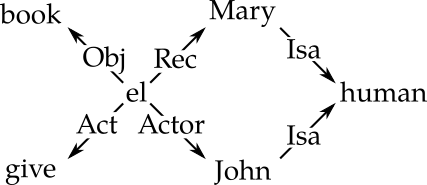
\includegraphics[scale=0.4]{figures/chapter7/semantic_net.png}
\caption{\label{fig:chap7_sem_net} The semantic network used to represent the assertion "\textit{John gives the book to Mary}". The element \textit{el} is used to represent the global event.}
\end{figure}

The general idea used in all the proposed approaches since Deliyanni is thus the creation of a \textbf{relation-class} that is instantiated to represent the n-ary relation. Then $n$ binary relations are created to link the $n$ entity to the relation-class instance. For a more global view of the different proposed patterns, you can refer to the survey~\cite{gangemi_2013_multi}.

For the use in ontology, no standard pattern has been approved by the W3C for the moment. However, a Working Group Note has been proposed for the standardisation of such relations in RDF and OWL~\cite{w3c_2006_defining}. In the note, two patterns are introduced with two variants for the first one.

The first pattern is based on the introduction of a new class for relation and works in the exact same way of the relation reification as illustrated in Figure~\ref{fig:chap7_w3c_p2}. The class \textit{Purchase} is a relation-class and its instance \textit{purchase\_1} is link the entities of the relation. Such pattern is said to be \textbf{without subject} as all the relation are oriented from the relation-class instance to the other entities.

\begin{figure}[ht!]
\centering
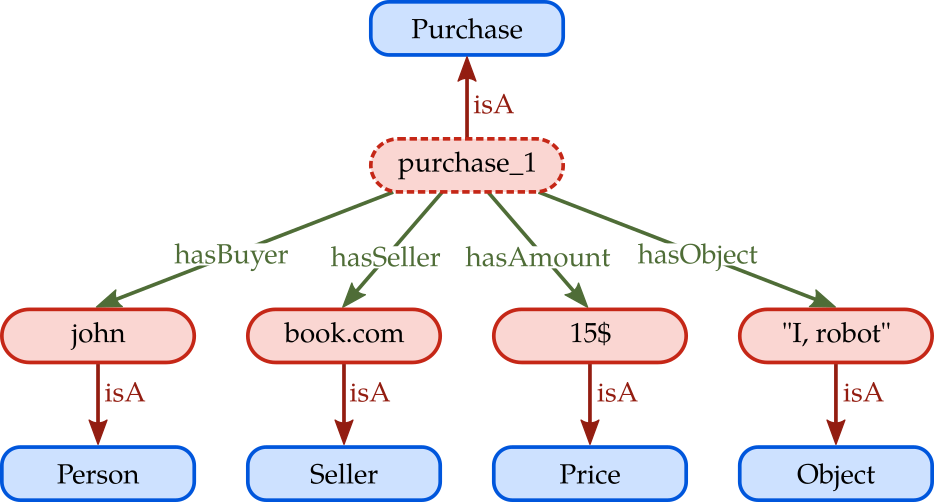
\includegraphics[scale=0.4]{figures/chapter7/w3c_p2.png}
\caption{\label{fig:chap7_w3c_p2} Ontological pattern 1 without subject proposed by the W3C Working Group. The describe assertion is "John buys a "I, robot" from books.com for \$15".}
\end{figure}

A variation of the first pattern is illustrated in Figure~\ref{fig:chap7_w3c_p1}. This variation is said to be \textbf{with subject}. The assertion described here is "Christine has a tumor with high probability". Here the subject of the relation is Christine. It is represented in the pattern by a relation oriented from Christine to the instance of the relation-class while the others are in the usual orientation. Such variation can be reproduced with the previous one by defining inverse relations. Defining the relation \textit{isBuyer} and \textit{isObject}, either John or the book can be the subject of the relation represented by \textit{purchase\_1}.

\begin{figure}[ht!]
\centering
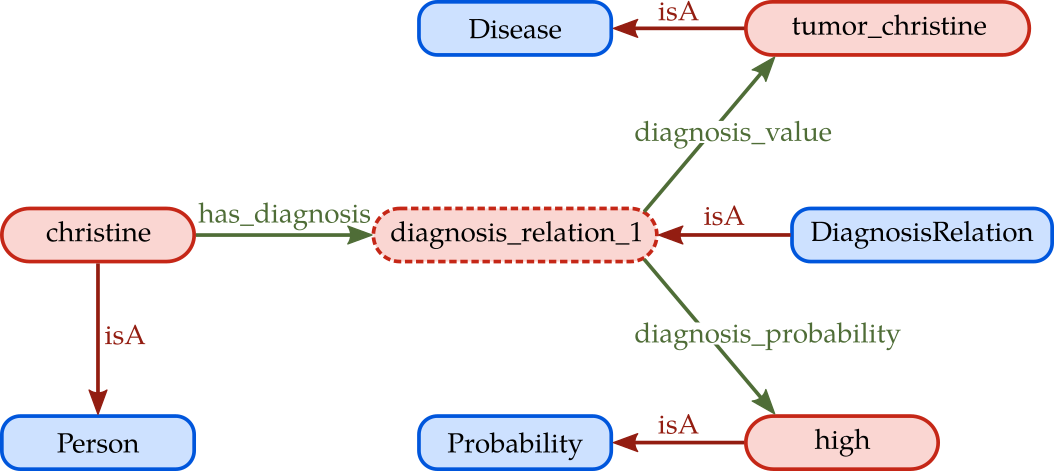
\includegraphics[scale=0.4]{figures/chapter7/w3c_p1.png}
\caption{\label{fig:chap7_w3c_p1} Ontological pattern 1 with subject proposed by the W3C Working Group. The describe assertion is "Christine has tumor with high probability".}
\end{figure}

The second pattern aims at representing lists. With the previous pattern, it is assumed that the properties involved in the binary relation are only used once to identify uniquely each element of the relation. Wanting to represent the assertion "United Airlines flight 3177 visits the following airports: LAX, DFW, and JFK" the first pattern would be not adapted. With this other pattern, we create several instances of the relation-class each linked to the next and to an entity of the n-ary relation as illustrated in Figure~\ref{fig:chap7_w3c_p3}. Because one of the binary relations go from an entity of the relation to an instance of the relation-class, it is said to be with subject. This second pattern is dedicated to the description of lists.

\begin{figure}[ht!]
\centering
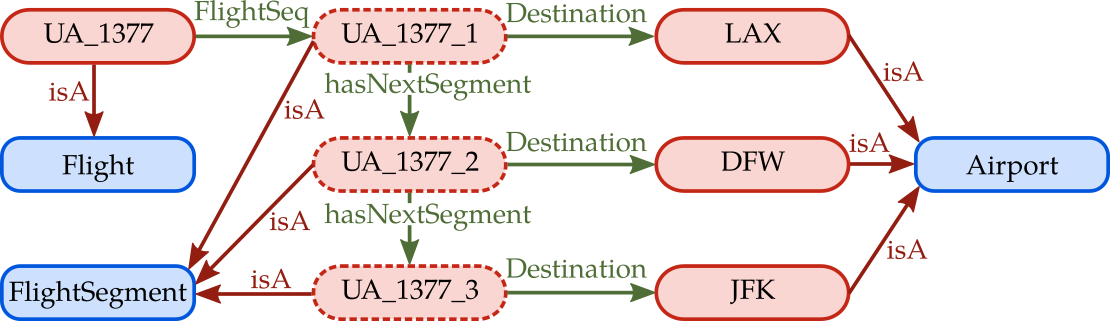
\includegraphics[scale=0.4]{figures/chapter7/w3c_p3.png}
\caption{\label{fig:chap7_w3c_p3} Ontological pattern 2 with subject proposed by the W3C Working Group. The describe assertion is "United Airlines flight 1377 visits the following airports: LAX, DFW, and JFK".}
\end{figure}

\section{Through the use of coumpound relations}

In the rest of the chapter, we consider the n-ary relations with arity $n > 2$ under the name \textbf{Compound Relations} (CR) because of the composition of binary relations to represent them on the principle of reification. The term relation will be used to speak about binary relations. We first define what is a CR in link with the ontology definition and on the base of the first pattern without subject, proposed by the Working Group Note. Then, we present an algorithm to pre-process them with the objective to facilitate their use in the REG algorithm.

\subsection{Defining a compound relation}

To define the structure of a Compound Relation we take the example of the purchase made by John on the website book.com to buy the book "I, Robot" at 15\$. This statement is graphically represented in Fig.~\ref{fig:chap7_cr}a and the underlying pattern in Fig.~\ref{fig:chap7_cr}b. To represent the compound relation, we start by creating a virtual entity (the instance of the relation-class) that will be the common link for all the relations involved in the compound relation. We call this instance entity the \textbf{Compound Entity} (CE). It is the dotted entity on Figure~\ref{fig:chap7_cr}, respectively $purchase\_1$ and $\indiv_c$. We consider as being part of the CR all the relations for which the CE is the subject: $(purchase\_1, has\_buyer, john)$. 

\begin{theorem} [Compound Relation]
\label{the:compound_relation}
For any $\indiv_c$ being a Coumpound Entity, a Coumpound Relation is defined by $R_c = \{ \relation_i\ |\  \relation_i = (\indiv_c, \property_i, \indiv_i), \forall \indiv_i \in \indivset\}$ meaning the set of relation composing it.
\end{theorem}

\begin{figure}[ht!]
\centering
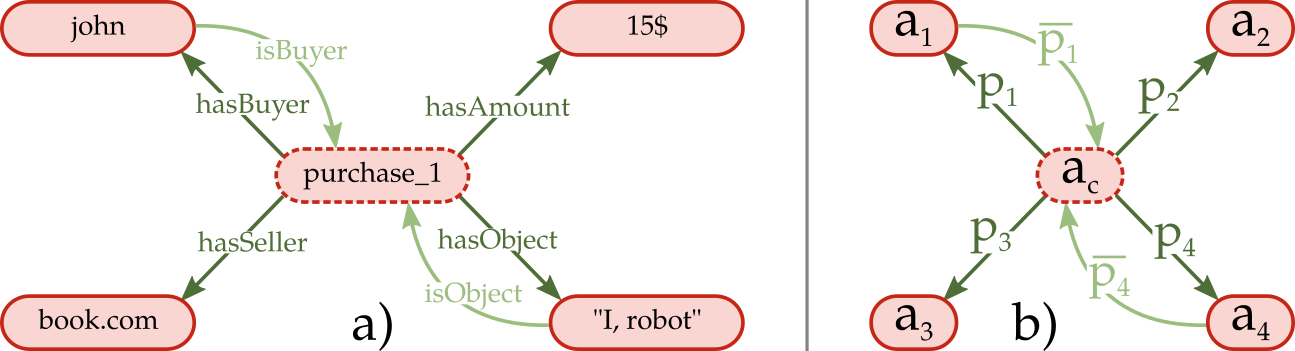
\includegraphics[width=\textwidth]{figures/chapter7/CR.png}
\caption{\label{fig:chap7_cr} The graphical representation of compound relations. The dotted entity at the center of each representation is the so-called compound entity. The outgoing edges are the properties involved in the compound relation. The entering and faded edges are the corresponding inverse properties if any. The compound relation a) describe the purchase made by \underline{John} on the website \underline{book.com} of the book \underline{"I, Robot"} at \underline{15\$}. The compound relation b) is the underlying pattern of the previous example.}
\end{figure}

Regarding the previous definition, because any entity of an ontology could be considered as a CE, many set of relations without a real link could be considered as a CR. To solve it, we could define an upper class common the all the CE, meaning the upper \textit{RelationClass}. However, what better defines a CR is that to speak about one of its involved entities through it, we have to use other relation of the CR. In other words, to speak about Sean Connery using the role of James Bond, we have to speak about "Gold Finger" rather than "Murder on the Orient Express" because even if he played in both films, he played the said role only in the first-mentioned film. At the difference, the relation representing his nationality can be used independently to other relations. To represent this verbal link, Giunti et .al \cite{giunti_2019_representing} introduce an \textit{parametric pattern} on top of n-ary relations (Compound Relations). Their parametric pattern for the purchase example is the following : \textit{"() bought a () from () for ()"}. While as humans we easily identify the place of each entity in the pattern, it is a more complex task for machines. This choice of pattern is explained by their complex representation where they assign a position to each involved relation. Regardless of the representation complexity, this kind of pattern raises two issues. First, the pattern describes the entire CR and not aims to describe one of the involved entity through the CR (e.g. "\textit{() who bought a () from () for ()}"). Second, the pattern necessary involved all the relations composing the CR, while in the context of the REG, we could only need a part of them (e.g. \textit{"() who bought a ()}" if John is the only one who bought this book in the present context).

\subsection{A light way of representing the verbal link}

To represent the verbal link, we also choose to use parametric patterns, patterns for short. The patterns are defined as labels in the ontology. A CR can have multiple labels (i.e. patterns) depending on the subject of the pattern and the involved relations in the verbal link. The labels are not directly applied to the CE but to a class, it's inheriting. This means that all the entities inheriting from a class having its labels respecting the pattern are CE. In a way, we define here a relation-class but one the only base of labels.

\begin{theorem} [Compound Entity]
\label{the:compound_relation}
Given $\omega$ being a pattern, an entity $\indiv_c$ is a Compound Entity iif $\exists \class \in \classset | (\indiv_c, \class) \in \inheritset \land \omega \in \tlabel{(\class)}$
\end{theorem}

An advantage of this solution is that we do not define any new specific concepts or properties in the ontology meaning that any pre-existing ontology can be updated to be used in the REG process with CR only by adding labels. Our patterns have the following form : $\{?\property_4\}\ bought\ on\ \{\property_3\}\ by\ \{\property_1\}$. This pattern directly integrates the properties which can be used to form the relations composing the CR.

Given a compound entity $a_c$ with the previous label, to generate a referring expression using it, the place-holder $\{\property_3\}$ should be replaced by a referring expression of an entity $\indiv_i$ where $\indiv_i$ is the object of a triple $(\indiv_c,\ \property3,\ \indiv_i)$. Because we assume that a property can only appear once in a CR, we know that there is only one such object $\indiv_i$. In our example, we have $\indiv_i = \indiv_3$ for the $a_c$ CE.
In this way, without predefined order, an algorithm can easily replace the place-holders by the RE of the entities $\indiv_i$ of the relations $(\indiv_c, \property_i, \indiv_i)$ of the CR.

Since we are in the context of REG, the CR will be used as a reference to one of the entities involved in the CR. This specific entity is called the \textbf{subject entity} of the CR. 
For a subject entity to exist, an inverse property $\overline{\rm \property_i}$ must exists in the way that $(\property_i, \overline{\property_i}) \in \invset$ and $\relation_i = (\indiv_i, \overline{\property_i}, \indiv_c) \in \relationset$. If $\indiv_i$ is the subject entity, $\property_i$ is thus the \textbf{subject property} of the CR and is prefixed with a question mark in the pattern. In the example of Figure~\ref{fig:chap7_cr}, only $\indiv_1$ and $\indiv_4$ (resp. John and the book) can be subject of the CR. In other words, only these entities can be referred through the use of this CR. Among all the labels available to speak about the CR, the usable ones to speak about an entity are the ones for which the corresponding property is the subject property (i.e. prefixed by a question mark in the patterns). This choice to not consider the first in the pattern has been made to be adapted to any language. Among the possible labels of List.\ref{lst:chap7_john_labels}, the patterns L1 to L5 could thus be used as a reference for $\indiv_4$ (the book in our example) while the patterns L6 and L7 could be used as a reference for $\indiv_1$ (John in our example).

\begin{lstlisting}[frame=single, caption={ A part of the label set of the purchase compound relation.}, label={lst:chap7_john_labels}, captionpos=b, style=Labels, mathescape=true]
L1 - {?$p_4$} bought on {$p_3$} at {$p_2$}
L2 - {?$p_4$} bought by {$p_1$}
L3 - {?$p_4$} bought on {$p_3$} by {$p_1$}
L4 - {$?p_4$} bought at {$p_2$} on {$p_3$} by {$p_1$}
L5 - {$?p_4$} bought at {$p_2$} by {$p_1$}
L6 - {$?p_1$} who bought {$p_4$}
L7 - {$?p_1$} who bought {$p_4$} on {$p_3$}
\end{lstlisting}

\subsection{A strategy to explore compund relations}

%In a graph exploration, an important parameter to avoid a combinatorial explosion is the branching factor. 

%Even if the full REG algorithm will be later in the paper, we have here to keep in mind that the main principle will be to explore a graph for which the edge will be relations of the ontology. An advantage of CR is that once we introduce a CR in the search algorithm we can directly know the relations involved in it. In this sub-section, our goal is thus to analyze the labels in the way to define the order in which the relations of the CR will be explored by the upper algorithm. By doing so, we will reduce its branching factor and thus avoid any combinatorial explosion of the REG algorithm.

\subsubsection{A naive startegy to explore compound relations}

\subsubsection{A advanced strategy to explore compound relations}


\section{Generating Referring Expression wit compound relations}

\subsection{Determining a referring expression validity}

\subsection{Exploring the compound relations}

\subsection{From tree to radix tree}


\section{Results}

\subsection{The actor playing James Bond}

\subsection{The desciption of past activities as compound relations}